\textbf{C.1. Thermoluminescence Dosimetry}

Many crystalline materials exhibit the phenomenon of thermoluminescence (TL). When such a crystal is irradiated, a very minute fraction of the absorbed energy is stored in the crystal lattice. Some of this energy can be recovered later as visible light if the material is heated. This phenomenon of the release of visible photons by thermal means is known as TL.

The arrangement for measuring the TL output is shown schematically in Figure 8.10. The irradiated material is placed in a heater cup or planchet, where it is heated for a reproducible heating cycle. The emitted light is measured by a photomultiplier tube (PMT), which converts light into an electrical current. The current is then amplified and measured by a recorder or a counter.

There are several TL phosphors available, but the most noteworthy are lithium fluoride (LiF), lithium borate (Li$_2$B$_4$O$_7$), and calcium fluoride (CaF$_2$). Their dosimetric properties are listed in Table 8.6. Of these phosphors, LiF is most extensively studied and most frequently used for clinical dosimetry. LiF in its purest form exhibits relatively little TL. But the presence of a trace amount of impurities (e.g., magnesium) provides the radiation-induced TL. These impurities give rise to imperfections in the lattice structure of LiF and appear to be necessary for the appearance of the TL phenomenon.

\subsection{TLD Personnel Monitoring Badge}

\begin{figure}[h!]
    \centering
    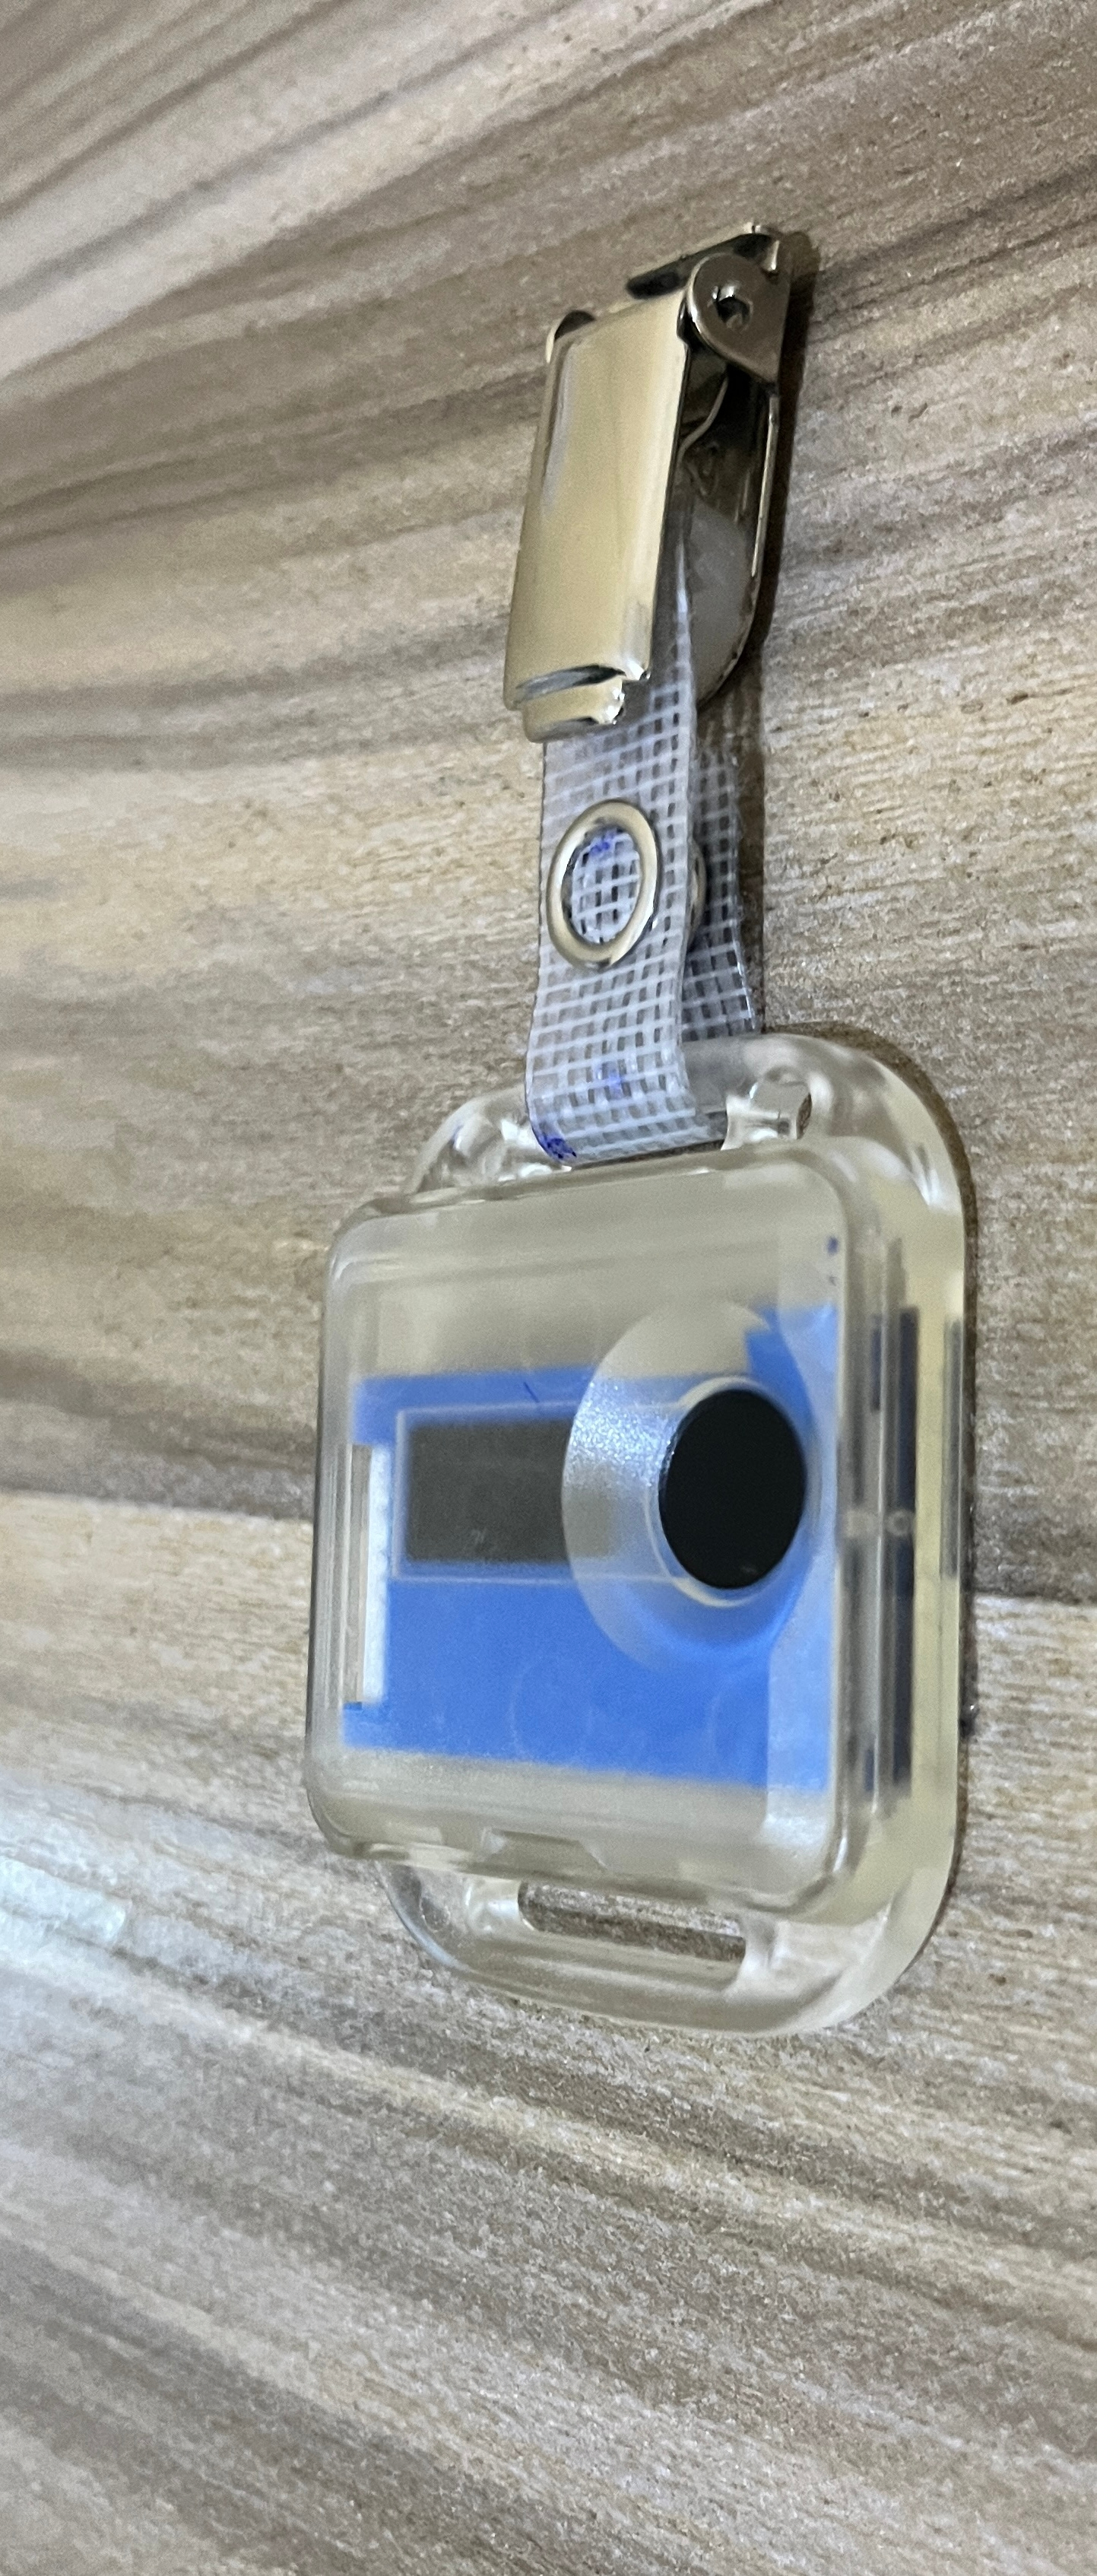
\includegraphics[width=0.4\textwidth]{Figures/TLD_Badge.jpg}
    \caption{A typical Thermoluminescent Dosimeter (TLD) personnel monitoring badge.}
    \label{fig:tld_badge}
\end{figure}

The Thermoluminescent Dosimeter (TLD) personnel monitoring badge is a crucial device used to measure an individual's accumulated exposure to ionizing radiation. In medical and industrial environments, these badges ensure occupational radiation safety and regulatory compliance by monitoring the cumulative dose received by staff, such as radiologists, technicians, and other medical personnel.

\subsubsection{Operating Principle}
The fundamental principle of a TLD badge is based on thermoluminescence. When the thermoluminescent material inside the badge is exposed to ionizing radiation (such as X-rays, gamma rays, or beta particles), electrons within the crystal lattice are excited and become trapped in metastable energy states (traps) caused by impurities or defects in the crystal. 

These electrons remain trapped until the material is heated in a controlled manner using a TLD reader. Upon heating, the trapped electrons acquire enough thermal energy to escape the traps and return to their ground state. During this de-excitation process, the energy is released in the form of visible light (luminescence). The intensity of the emitted light is measured by a photomultiplier tube and is directly proportional to the amount of radiation dose absorbed by the dosimeter material.

\subsubsection{Materials Used}
Several thermoluminescent materials are utilized in personnel monitoring depending on the required sensitivity and energy response. The two most common materials used for medical applications are:

\begin{enumerate}
    \item \textbf{Calcium Sulfate doped with Dysprosium (CaSO$_4$:Dy)}: 
    This is the most widely used material for TLD badges in India (standardized by BARC) and many other countries. 
    \begin{itemize}
        \item \textbf{High Sensitivity}: It is known for its exceptionally high sensitivity, particularly to low-energy photons, making it ideal for personnel monitoring where low dose detection is critical.
        \item \textbf{Form Factor}: It is typically used in the form of CaSO$_4$:Dy phosphor embedded in Teflon discs.
        \item \textbf{Energy Response}: Due to its relatively high effective atomic number ($Z_{eff} \approx 15.6$), it shows a significant over-response to low-energy X-rays compared to tissue. To compensate for this energy dependence, the TLD badge cassette is fitted with specific metallic filters (e.g., Copper and Aluminum) to flatten the energy response and accurately estimate the tissue dose.
    \end{itemize}

    \item \textbf{Lithium Fluoride (LiF)}:
    Lithium Fluoride, often doped with Magnesium and Titanium (LiF:Mg,Ti, commercially known as TLD-100) or Magnesium, Copper, and Phosphorus (LiF:Mg,Cu,P), is another highly valued material globally.
    \begin{itemize}
        \item \textbf{Tissue Equivalence}: Its primary advantage is its near tissue-equivalent effective atomic number ($Z_{eff} \approx 8.2$, compared to 7.4 for soft tissue). This means its radiation absorption characteristics closely match those of human tissue across a wide range of photon energies.
        \item \textbf{Sensitivity}: While traditional LiF:Mg,\allowbreak Ti is less sensitive than CaSO$_4$:\allowbreak Dy, the newer LiF:Mg,\allowbreak Cu,\allowbreak P variants offer extremely high sensitivity and low fading at room temperature, making them excellent for precise medical dosimetry.
    \end{itemize}
\end{enumerate}

\subsubsection{Badge Design and Filters}
A typical TLD badge wrapper (cassette) consists of multiple regions or "windows" containing different filters (such as open window, plastic filter, and metallic filters like Cu or Al). The dosimeter discs (e.g., three CaSO$_4$:Dy discs) are positioned behind these filters. 
\begin{itemize}
    \item The different filters allow for the discrimination between different types of radiation (e.g., beta vs. gamma) and different energy ranges.
    \item By comparing the readings from the discs behind different filters, the radiation quality and the accurate whole-body dose ($H_p(10)$) and skin dose ($H_p(0.07)$) can be evaluated.
\end{itemize}

HI